\documentclass[10pt]{book}
\usepackage[utf8]{inputenc}
\usepackage[italian]{babel}
\usepackage{multicol}
\usepackage[bookmarks]{hyperref}
\usepackage[a4paper, total={18cm, 25cm}]{geometry}
\usepackage{tikz}
\usepackage{color}
\definecolor{mygray}{rgb}{0.5,0.5,0.5}
\usepackage{listings}
\usepackage{mathrsfs}
\lstset{
	language=Matlab,
	commentstyle=\color{mygray}
}
\usepackage{graphicx}
\usepackage{makecell}
\graphicspath{ {./img/} }
\usepackage{color}

\begin{document}
\renewcommand*\contentsname{Indice}
\title{Calcolo Numerico}
\author{Federico Matteoni}
\date{A.A. 2019/20}
\maketitle
\tableofcontents
\pagebreak
\section*{Introduzione}
Prof.: Luca Gemignani
\paragraph{Calcolo Numerico} Metodi numerici per risolvere problemi matematici con il calcolatore. In questo corso ce ne occuperemo dal punto di vista numerico, perché metodi di risoluzione diversi performano in maniera diversa sulla macchina. Cerchiamo di capire quali sono i metodi di interesse e cosa aspettarci dalla loro implementazione.\\
Il \textbf{metodi numerici approssimano la soluzione di problemi matematici}.\\
Inoltre, il computer \textbf{impatta} sul calcolo perché lavora con approssimazioni dei numeri, che su moli elevate di dati e di elaborazioni finiscono per perturbare il risultato ottenuto.
\paragraph{Tipici problemi} $$Ax = b$$ $$Ax = \lambda x$$ $$f(x) = 0$$ $$\int_a^bf(x) dx$$
\paragraph{Matlab} Matrix Laboratory, strumento di implementazione per verificare e constatare i risultati teorici.
\paragraph{Informazioni d'esame} Compitini, che se complessivamente passati rendono l'orale facoltativo. In alternativa, appelli scritti + orale.
\pagebreak
\chapter{Aritmetica di macchina}
Modello per capire cosa aspettarci dal punto di vista degli errori dell'esecuzione.
\paragraph{Esempio} Per calcolare il limite $$\lim_{x\to\infty} \sqrt{x + 1} - \sqrt{x}$$ ottengo un caso indeterminato ($\infty - \infty$). Posso semplificare l'espressione ad esempio razionalizzando, e con pochi passaggi ottengo la seguente uguaglianza $$\sqrt{x + 1} - \sqrt{x} = \frac{1}{\sqrt{x + 1} + \sqrt{x}}$$ Quindi dal punto di vista matematico, le due espressioni sono equivalenti. Ciò \textbf{non è sempre vero per la rappresentazione ed il calcolo in macchina}: le due espressioni forniranno risultati completamente diversi. Si rende \textbf{necessario}, quindi, \textbf{capire quale metodo si comporta meglio} rispetto agli altri.
\section{Rappresentazione in macchina}
\paragraph{Rappresentare i numeri} Siamo comunemente abituati a rappresentare un numero in diverse forme.\\
Ad esempio, $0.1 = \frac{1}{10} = 10 \cdot 0.01$. In generale, per ogni numero ho diversi metodi di rappresentazione $\Rightarrow$ In macchina dobbiamo poter \textbf{rappresentare i numeri in maniera univoca}.
\paragraph{Base di numerazione} $B \in N, B > 1$, poiché in base 1 non si può contare.\\Una base $B$ ha cifre nell'insieme $\{0, 1, \ldots, B - 1\}$
\paragraph{Teorema} Dato $x \in R$, con $x \neq 0$\\$\exists!\:\:(\{d_i\}_{i \geq 1}$ con $d_1 \neq 0$ e $d_i$ non definitivamente uguali a $B - 1) \wedge (p \in Z) \:\:\vline\:\: x = segno(x)\:\cdot\:B^p\:\cdot\:\sum_{i=1}^\infty d_i \cdot B^{-i}$
\begin{list}{}{Considerazioni}
	\item Se $x \in C$ allora viene rappresentato come coppia di numeri reali, quindi il problema si riconduce sempre alla loro rappresentazione
	\item Lo $0$ viene rappresentato in modo speciale, poiché non esiste una sua rappresentazione normalizzata
	\item ${d_i}_{i \geq 1}$ è una \textbf{successione} di cifre
	\item La rappresentazione è \textbf{normalizzata} se $d_1 \neq 0$, cioè se la prima cifra è diversa da 0
	\item Non può avere tutte cifre uguali a $B-1$ da un certo punto in poi, la rappresentazione "collassa" al numero successivo
	\item $p$ è detto \textbf{esponente}
	\item $\sum_{i=1}^\infty d_i \cdot B^{-i}$ è detta \textbf{mantissa}
	\item Questa rappresentazione si chiama \textbf{in virgola mobile} o \textbf{floating point}
\end{list}
\begin{center}
\begin{tikzpicture}
  \draw [draw=black, align=center] (0, 0) rectangle ++(1, 1) node[midway] {Segno};
  \draw [draw=black, align=center] (1, 0) rectangle ++(2, 1) node[midway] {Esponente};
  \draw [draw=black, align=center] (3, 0) rectangle ++(4, 1) node[midway] {Mantissa};
\end{tikzpicture}
\end{center} %credits: loures
\pagebreak
\paragraph{Esempi} Ponendo $B = 10$
\begin{list}{}{}
	\item $x = 0.01 \Rightarrow x = +10^{-1}\cdot(0.1)$
	\item $x = 1.35 \Rightarrow x = +10^1\cdot(0.135)$
	\item $x = 0.0023 \Rightarrow x = +10^{-2}\cdot(0.23)$
\end{list}
\paragraph{Numeri di Macchina} Nei computer ho \textbf{registri di lunghezza finita}, quindi essi vengono partizionati: una parte viene riservata alla rappresentazione dell'\textbf{esponente} e il resto alla rappresentazione della \textbf{mantissa}. L'\textbf{insieme dei numeri di macchina} F è quindi così definito
$$F(B, t, m, M) = \{\pm B^p \cdot \sum_{i=1}^t d_i \cdot b^{-i}\:\:\vline\:\: d_1 \neq 0 \wedge -m \leq p \leq M\} \cup \{0\}$$
\begin{list}{}{dove}
	\item $t$ sono le \textbf{cifre della mantissa}
	\item L'esponente p è compreso tra i valori $-m$ e $M$
	\item Lo 0 è incluso ma rappresentato a parte
\end{list}
\paragraph{Esempio} Ipotizzando di usare registri da 32 bit, posso stanziare 8 bit per l'esponente $p$ (quindi 1 bit per il segno e 7 bit per il valore) e i restanti 24 bit per la mantissa (1 per il segno, 23 per il valore). Quanti numeri posso rappresentare?
\begin{list}{}{}
	\item $p$ di 7 bit $\Rightarrow 2^7 - 1 = 127 \Rightarrow -127 \leq p \leq 127$ ma lo 0 è rappresentato due volte
	\item $x = \pm2^p \sum_{i=1}^23 d_i \cdot 2^{-1}$, con $d_i \in \{0, 1\}$, $d_1 \neq 0 \Rightarrow d_1 = 1$ sempre
\end{list}
Vedremo che con una serie di accorgimenti è possibile aumentare i numeri esattamente rappresentabili.\\\\
Dato quindi $F(B, t, m, M)$, osservo che:
\begin{list}{}{}
	\item $F(B, t, m, M)$ ha cardinalità finita $N = 2B^{t-1}(B - 1)(M + m + 1) + 1$
	\item Se $x \in F(B, t, m, M) \wedge x \neq 0 \Rightarrow \omega = B^{-m-1} \leq |x| \leq B^M(1 - B^{-t}) = \Omega$\\
	Quindi non è possibile rappresentare esattamente numeri non nulli minori di $\omega$. Si può introdurre una rappresentazione \textbf{denormalizzata} quando $p = -m$: la condizione $d_1 \neq 0$ può essere abbandonata e posso così rappresentare numeri positivi e negativi compresi in modulo tra $B^{-m-t}$ e $B^{-m}(B^{-1} - B^{-t})$\\
	Analogamente se $p = M$ si introducono rappresentazioni speciali per i simboli $\pm\infty$ e NaN (\textbf{not a number}).
\end{list}
\subsection{Aritmetica di Macchina}
La rappresentazione di un numero $x \in R, x \neq 0$ in macchina significa \textbf{approssimare} $x$ con un numero\\$\overline{x} \in F(B, t, m, M)$ commettendo un \textbf{errore relativo} di rappresentazione $$\epsilon_x = \frac{\overline{x} - x}{x} = \frac{\eta_x}{x}, x \neq 0$$ quanto più piccolo possibile in valore assoluto. La quantità $\eta_x = \overline{x} - x$ è detta \textbf{errore assoluto} della rappresentazione.\\
L'errore relativo è importante per la \textbf{valutazione qualitativa} dell'errore: nelle misurazioni astronomiche un errore assoluto di 1 cm è \textit{qualitativamente diverso} da un errore assoluto di 1 cm nella misurazione di un tavolo.\\\\
Dato $x \in R, x \neq 0$, distinguiamo due casi:
\begin{enumerate}
	\item $|x| < \omega$ (\textbf{underflow}) oppure $|x| > \Omega$ (\textbf{overflow})
	\item $\omega \leq |x| \leq \Omega$
\end{enumerate}
\pagebreak
Nel secondo caso abbiamo quattro tecniche di approssimazione:
\begin{enumerate}
	\item \textbf{Arrotondamento}: $x$ approssimato con il numero rappresentabile $\overline{x}$ più vicino
	\item \textbf{Troncamento}: $x$ approssimato con il più grande numero rappresentabile $\overline{x}$ tale che $|\overline{x}| \leq |x|$
	\item \textit{Round toward $+\infty$}: $x$ approssimato al più piccolo numero rappresentabile maggiore del dato
	\item \textit{Round toward $-\infty$}: $x$ approssimato al più grande numero rappresentabile minore del dato
\end{enumerate}
Per semplicità considereremo una macchina che opera per troncamento sull'insieme $F(B, t, m, M)$.\\
Indicheremo con $trn(x) = \overline{x}$ il risultato dell'approssimazione di $x$ con troncamento e più in generale $fl(x)$ l'\textbf{approssimazione in macchina del dato $x$} nel sistema floating point considerato.
\paragraph{Teorema} Sia $x \in R$ con $\omega \leq |x| \leq \Omega$. Si ha $$|\epsilon_x| = |\frac{trn(x) - x}{x}| \leq u = B^{1-t}$$
Si osserva che:
\begin{list}{}{}
	\item $u = B^{1-t}$ è detta \textbf{precisione di macchina} ed è \textbf{indipendente dalla grandezza del numero}, ma è caratteristica dell'aritmetica floating point, dell'insieme dei numeri rappresentabili e dalla tecnica di approssimazione. Se ad esempio si opera con arrotondamento, $u$ si dimezza.
	\item Per valutare la precisione di macchina possiamo determinare il più piccolo numero di macchina maggiore di 1. Dato $x$ tale numero, abbiamo $x - 1 = |x - 1| = B^{1-t}$ essendo $1 = B^1 \cdot B^{-1}$ rappresentato con esponente $p = 1$. Il seguente script MatLab fornisce il valore richiesto:
	\begin{lstlisting}
		eps = 0.5;
		eps1 = eps + 1;
		while(eps > 1)
			eps = 0.5 * eps;
			eps1 = eps + 1;
		end
		eps = 2 * eps;
	\end{lstlisting}
	\item Dal teorema si ricava che dato $x \in R$, in assenza di overflow/underflow, vale $fl(x) = x(1 + \epsilon_x)$ con $|\epsilon_x| \leq u$.\\
	Questa relazione esprime il modo in cui viene descritto generalmente il legame tra numero reale e sua rappresentazione in macchina.
\end{list}
\subsection{Operazioni di Macchina}
Per le \textbf{operazioni aritmetiche} in un sistema floating point si pone un analogo problema di approssimazione, in quanto \textbf{il risultato di un'operazione eseguita tra due numeri di macchina in generale non sarà un numero di macchina}.
\paragraph{Operazioni} Indichiamo con $\oplus$, $\ominus$, $\otimes$, $\oslash$ le \textbf{operazioni aritmetiche di macchina} corrispondenti relativamente all'addizione, sottrazione, prodotto e divisione. Si richiede che le operazioni siano interne all'insieme dei numeri di macchina. Una ragionevole definizione, derivata dal teorema precedente e in assenza di overflow/underflow, risulta: $$\forall a, b \in F(B, t, m, M), a \oplus b = fl(a + b) = (a + b)(1 + \epsilon_1), |\epsilon_1| \leq u$$ con $\epsilon_1$ detto  \textbf{errore locale dell'operazione}. Sempre in assenza di overflow/underflow, se $a, b \in R$ si ha $$fl(a + b) = fl(a)\oplus fl(b) = (a(1 + \epsilon_a) + b(1 + \epsilon_b))(1 + \epsilon_1) \doteq (a + b) + a\epsilon_a + b\epsilon_b + (a + b)\epsilon_1$$ dove con $\doteq$ si indica che l'eguaglianza vale \textbf{considerando le sole componenti lineari negli errori} e trascurando le componenti di ordine superiore (\textbf{analisi al primo ordine dell'errore}), in virtù del fatto che gli $\epsilon$ sono quantità piccole $0 < \epsilon < 1$, quindi trascurabili negli ordini superiori al primo.\\
Si ottiene che, in assenza di overflow/underflow, se $a, b \in R, a + b \neq 0$, allora $$\frac{fl(a + b) - (a + b)}{a + b} \doteq \frac{a}{a + b}\epsilon_a + \frac{b}{a + b}\epsilon_b + \epsilon_1$$ che esprime la dipendenza dell'errore totale commesso nel calcolo della somma tra due numeri reali rispetto agli errori generati dall'approssimazione dei dati iniziali (\textbf{errore inerente}) e agli errori generati dall'algoritmo di calcolo (\textbf{errore algoritmico}) visto come sequenza di operazioni artimetiche.\\
\pagebreak
\paragraph{Esempio}
Analizziamo cosa succede in macchina quando proviamo a calcolare $f(x) = x^2 - 1 = (x - 1)(x + 1)$. La \textbf{prima situazione di errore} sia ha sulla rappresentazione di $x$ che, \textbf{in generale}, \textbf{non è un numero di macchina}.$$x \rightarrow \tilde{x} = x(1 + \epsilon_x)$$ con $|\epsilon_x| \leq u$. Inoltre, sempre in generale, \textbf{le operazioni aritmetiche non sono operazioni di macchina} $$f(x) = (\tilde{x} \otimes \tilde{x}) \ominus 1 = (\tilde{x} \ominus 1)\otimes(\tilde{x} \oplus 1)$$Poniamo $g_1(x) = (\tilde{x} \otimes \tilde{x}) \ominus 1$ e $g_2(x) = (\tilde{x} \ominus 1)\otimes(\tilde{x} \oplus 1)$. La formula per l'\textbf{errore totale} dell'operazione è $$\epsilon_{tot1} = \frac{g_1(x) - f(x)}{f(x)}$$ $$\epsilon_{tot2} = \frac{g_2(x) - f(x)}{f(x)}$$ Sviluppiamo $g_1(x)$

$$g_1(x) = ((x(1+\epsilon_x)\cdot x(1 + \epsilon_x))(1 + \epsilon_1) - 1)(1 + \epsilon_2) \doteq$$
$$\doteq (x^2(1 + 2\epsilon_x)(1 + \epsilon_1) - 1)(1 + \epsilon_2) \doteq$$
$$\doteq (x^2 ((1 + 2\epsilon_x + \epsilon_1) - 1)(1 + \epsilon_2) \doteq$$
$$\doteq x^2(1 + 2\epsilon_x + \epsilon_1 + \epsilon_2) - (1 + \epsilon_2) =$$
$$= (x^2 - 1) + 2x^2\epsilon_x + x^2\epsilon_1 + (x^2 - 1)\epsilon_2 = g_1(x)$$
$$|\epsilon_i| \leq u$$ Quindi, portando al primo membro dell'uguaglianza $\epsilon_{tot1} = \frac{g_1(x) - f(x)}{f(x)}$ tutti i fattori $(x^2 - 1) = f(x)$ si ottiene $$\epsilon_{tot1} = \frac{2x^2}{x^2 - 1}\epsilon_x + \frac{x^2}{x^2 - 1}\epsilon_1 + \epsilon_2$$ Si evince che \textbf{l'errore totale è la somma di due componenti}:
\begin{list}{}{}
	\item \textbf{Errore inerente} o inevitabile: l'\textbf{errore di rappresentazione di $x$}, che vale 0 se $x$ è numero di macchina ed è \textbf{proprietà della funzione}. Nell'esempio, $\epsilon_{in} = \frac{2x^2}{x^2 - 1}\epsilon_x$.\\
	Se l'errore inerente è piccolo si dice che \textbf{la funzione è numericamente stabile}, viceversa è \textbf{numericamente instabile}.
	\item \textbf{Errore algoritmico}, locale all'operazione e \textbf{proprietà dell'algoritmo}. Nell'esempio, $\epsilon_{alg} = \frac{x^2}{x^2 - 1}\epsilon_1 + \epsilon_2$.\\
	Se è piccolo, si dice che l'\textbf{espressione è ben condizionata} e \textbf{poco sensibile rispetto alla perturbazione}. Viceversa, è \textbf{mal condizionata}.
\end{list}
Sviluppiamo ora $g_2(x)$ (gli errori $\delta_i$ sono analoghi agli $\epsilon_i$, si usa una notazione differente per evidenziare che hanno valori diversi, esseno propri del calcolo e dei valori usati in esso)
$$g_2(x) = ((x(1 + \epsilon_x) - 1)(1 + \delta_1))((x(1 + \epsilon_x) + 1)(1 + \delta_2))(1 + \delta_3) \doteq$$
$$\doteq (x^2(1 + \epsilon_x)^2 - 1)(1 + \delta_1 + \delta_2 + \delta_3) \doteq$$
$$\doteq (x^2(1 + 2\epsilon_x) - 1)(1 + \delta_1 + \delta_2 + \delta_3) =$$
$$= x^2(1 + 2\epsilon_x + \delta_1 + \delta_2 + \delta_3) - (1 + \delta_1 + \delta_2 + \delta_3) =$$
$$= (x^2 - 1) + 2x^2\epsilon_x + (x^2 - 1)(\delta_1 + \delta_2 + \delta_3) = g_2(x)$$
$$|\epsilon_x| \leq u, |\delta_i| \leq u$$
Come prima, porto gli $f(x)$ al primo membro dell'uguaglianza $\epsilon_{tot2} = \frac{g_2(x) - f(x)}{f(x)}$ e ottengo
$$\epsilon_{tot2} = \frac{2x^2}{x^2 - 1}\epsilon_x + \delta_1 + \delta_2 + \delta_3$$
\pagebreak

\begin{list}{}{Notiamo come}
	\item $\epsilon_{in} = \frac{2x^2}{x^2 - 1}\epsilon_x$, come il calcolo precedente. Infatti, ripetiamo, l'errore inerente è una proprietà della funzione e non di come essa viene calcolata
	\item $\epsilon_{alg} = \delta_1 + \delta_2 + \delta_3$, diverso poiché abbiamo seguito un calcolo differente
\end{list}
Per poter comparare i due algoritmi e scegliere il migliore, analizziamo gli errori algoritmici. L'analisi \textbf{va eseguita in valore assoluto}, poiché non si ha alcuna informazione sul segno degli errori, seguendo quindi le regole di comparazione dei valori assoluti:
\begin{list}{}{}
	\item $|a + b| \leq |a|\:+\:|b|$
	\item $|a\cdot b| = |a|\cdot|b|$
\end{list}
$$\epsilon_{alg1} = |\frac{x^2}{x^2 - 1}\epsilon_1 + \epsilon_2| \leq |\frac{x^2}{x^2 - 1}\epsilon_1| + |\epsilon_2| = |\frac{x^2}{x^2 - 1}|\cdot|\epsilon_1| + |\epsilon_2| \leq \frac{x^2}{|x^2 - 1|}u + u = (\frac{x^2}{|x^2 - 1|} + 1)u$$
$$\epsilon_{alg2} = |\delta_1 + \delta_2 + \delta_3| \leq |\delta_1| + |\delta_2| + |\delta_3| \leq 3u$$
In $\epsilon_{alg1}$, quindi, l'errore algoritmo è minore o uguale a $(\frac{x^2}{|x^2 - 1|} + 1)u$, che però diventa arbitrariamente grande quando $x$ si avvicina ad 1. Il secondo algoritmo è dunque \textbf{preferibile}, poiché l'\textbf{errore algoritmico è limitato}.
\paragraph{Esempio} Calcoliamo ora l'espressione $f(x) = x^2 + 1$. Poniamo $g(x) = (\tilde{x} \otimes \tilde{x}) \oplus 1$ e sviluppiamo, ottenendo $$g(x) \doteq x^2(1 + 2\epsilon_x + \epsilon_1 + \epsilon_2) + (1 + \epsilon_2)$$
L'errore totale è quindi
$$\epsilon_{tot} = \frac{g(x) - f(x)}{f(x)} = \frac{2x^2}{x^2 + 1}\epsilon_x + \frac{x^2}{x^2 + 1}\epsilon_1 + \epsilon_2$$ Studiamo le componenti
$$|\epsilon_{in} = |\frac{2x^2}{x^2 + 1}\epsilon_x| = |\frac{2x^2}{x^2 + 1}|\cdot|\epsilon_x| \leq \frac{2x^2}{x^2 + 1}u \leq 2u$$ perché $\frac{x^2}{x^2 + 1} \leq 1$. La funzione quindi \textbf{non è suscettibile rispetto alle perturbazioni dei dati in ingresso} ed è \textbf{ben condizionata}.
$$\epsilon_{alg} = |\frac{x^2}{x^2 + 1}\epsilon_1 + \epsilon_2| \leq |\frac{x^2}{x^2 + 1}\epsilon_1| + |\epsilon_2| = \frac{x^2}{x^2 + 1}|\epsilon_1| + |\epsilon_2| \leq |\epsilon_1| + |\epsilon_2| \leq 2u$$ Quindi l'algoritmo è \textbf{numericamente stabile} perché la componente dell'errore algoritmo è piccola ($\leq 2u$). Questo è il caso migliore che può capitare: \textbf{funzione ben condizionata} e \textbf{algoritmo numericamente stabile}.\\\\
Succede perché non vi è la sottrazione al numeratore. La sottrazione, in macchina, lavora usando molte delle cifre "sporche" della mantissa, cioè quelle che fanno parte del rumore e dell'errore di rappresentazione. Si chiama \textbf{errore di cancellazione}.
\subsection{Errore Inerente}
\paragraph{Definizione} Si dice \textbf{errore inerente} o \textbf{inevitabile} generato nel calcolo di $f(x) \neq 0$ la quantità $$\epsilon_{in} = \frac{f(\tilde{x}) - f(x)}{f(x)}$$
Osserviamo che l'errore inerente è una \textbf{proprietà della funzione}, ovvero del problema matematico, e misura la \textbf{sensibilità rispetto alla perturbazione del dato iniziale}. Quindi, è indipendente dall'algoritmo di calcolo.\\
Se l'errore inerente è qualitativamente elevato in valore assoluto, diciamo che \textbf{il problema matematico è mal condizionato}, altrimenti si dice che è \textbf{ben condizionato}.
\subsection{Errore Algoritmico}
\paragraph{Definizione} Si dice \textbf{errore algoritmico} generato nel calcolo di $f(x) \neq 0$ la quantità $$\epsilon_{alg} = \frac{g(\tilde{x}) - f(\tilde{x})}{f(\tilde{x})}$$
Osserviamo che l'errore algoritmico è \textbf{dipendente dall'algoritmo utilizzato}: la funzione $g$ dipende dall'algoritmo usato per calcolare $f(x)$. In generale, \textbf{differenti algoritmi conducono a differenti errori algoritmici}.\\
Se l'errore algoritmico è qualitativamente elevato in valore assoluto si dice che \textbf{l'algoritmo è numericamente instabile}, altrimenti si dice che è \textbf{numericamente stabile}.
\pagebreak
\subsection{Errore Totale}
\paragraph{Definizione} Si dice \textbf{errore totale} generato nel calcolo di $f(x) \neq 0$ mediante l'algoritmo specificato da $g$ la quantità $$\epsilon_{tot} = \frac{g(\tilde{x}) - f(x)}{f(x)}$$ L'errore totale misura la \textbf{differenza relativa tra l'output atteso e l'output effettivamente calcolato}.
\paragraph{Teorema} In un analisi al primo ordine, vale $$\epsilon_{tot} = \epsilon_{in} + \epsilon_{alg}$$
\subparagraph{Dim} $$\epsilon_{tot} = \frac{g(\tilde{x}) - f(x)}{f(x)} = \frac{f(\tilde{x}) - f(\tilde{x})}{f(\tilde{x})}\cdot\frac{f(\tilde{x})}{f(x)} + \frac{f(\tilde{x}) - f(x)}{f(x)} = \epsilon_{alg}(1 + \epsilon_{in}) + \epsilon_{in} \doteq \epsilon_{alg} + \epsilon_{in}$$
Viene espresso il fatto che nel calcolo di una funzione razione, in un'analisi al primo ordine, le due fonti di generazione d'errore forniscono contributi separati che possono essere analizzati indipendentemente.\\
L'obiettivo dell'analisi numerica è \textbf{trovare algoritmi numericamente stabili per problemi ben condizionati}.
\section{Tecniche per l'Analisi degli Errori}
\subsection{Coefficiente di Amplificazione}
Dalla seguente relazione $$\epsilon_{in} = \frac{f(\tilde{x}) - f(x)}{f(x)} = \frac{f(\tilde{x}) - f(x)}{\tilde{x} - x}\cdot\frac{x}{f(x)}\cdot\frac{\tilde{x} - x}{x}$$ si ricava che la \textbf{differenziabilità di $f(x)$ è essenziale} per il controllo dell'errore inerente. Se assumiamo che $f(x)$ è derivabile due volte e continua in $(a, b)$, allora vale lo sviluppo di Taylor $$f(\tilde{x}) = f(x) + f'(x)(\tilde{x} - x) + \frac{f''(\xi)}{2}(\tilde{x} - x)^2,\:\:\:\:\:\:|\xi - x| \leq |\tilde{x} - x| $$ da cui si ottiene $$ \epsilon_{in} = \frac{f(\tilde{x}) - f(x)}{f(x)} \doteq \frac{f'(x)}{f(x)}x\epsilon_x = c_x\epsilon_x,\:\:\:\:\:\:c_x = \frac{f'(x)}{f(x)}x $$
La quantità $c_x = c_x(f) = \frac{f'(x)}{f(x)}x$ è detta \textbf{coefficiente di amplificazione} e fornisce una \textbf{misura del condizionamento del problema}.\\
In generale, se $f$ : $\Omega \rightarrow R$ è definita su un insieme aperto di $R^n$, differenziabile due volte su $\Omega$ ed il segmento di estremi $\tilde{\textbf{x}}$ e $\textbf{x}$ è contenuto in $\Omega$ allora vale
$$ \epsilon_{in} = \frac{f(\tilde{\textbf{x}}) - f(\textbf{x})}{f(\textbf{x})} \doteq \frac{1}{f(\textbf{x})}\sum_{i=1}^n \frac{\partial f}{\partial x_i}(\textbf{x})x_i\epsilon_{x_i} = \sum_{i=1}^n c_{x_i}(f)\epsilon_{x_i}$$
con $$c_{x_i}(f) = \frac{1}{f(\textbf{x})}\frac{\partial f}{\partial x_i}(\textbf{x})x_i,\:\:\:\:\:\:1 \leq i \leq n$$
detti \textbf{coefficienti di amplificazione della funzione $f$ rispetto alla variabile $x_i$}.
\subparagraph{Esempio} per $f(x) = (x^2 + 1)/x$ si ha $$c_x = \frac{2 - (x^2 + 1)}{x^2}\cdot \frac{x}{x^2 + 1}\cdot x = \frac{x^2 - 1}{x^2 + 1}$$ e poiché $|c_x| \leq 1$ il problema risulta ben condizionato.
\subsubsection{Coefficienti}
Per le operazioni aritmetiche si ottiene
$$f(x, y) = x + y\:\:\:\:\:\:\epsilon_{in} \doteq c_x\epsilon_x + c_y\epsilon_y\:\:\:\:\:\:c_x=\frac{x}{x + y}\:\:\:\:c_y = \frac{y}{x + y}$$

$$f(x, y) = x - y\:\:\:\:\:\:\epsilon_{in} \doteq c_x\epsilon_x + c_y\epsilon_y\:\:\:\:\:\:c_x=\frac{x}{x - y}\:\:\:\:c_y = -\frac{y}{x - y}$$

$$f(x, y) = x \cdot y\:\:\:\:\:\:\epsilon_{in} \doteq c_x\epsilon_x + c_y\epsilon_y\:\:\:\:\:\:c_x= 1\:\:\:\:c_y = 1$$

$$f(x, y) = \frac{x}{y}\:\:\:\:\:\:\epsilon_{in} \doteq c_x\epsilon_x + c_y\epsilon_y\:\:\:\:\:\:c_x= 1\:\:\:\:c_y = -1$$
Ne segue, come visto in precedenza, che la sottrazione di due numeri vicini tra loro è potenziale causa di elevata amplificazione degli errori relativi (\textbf{cancellazione numerica}). Si nota anche come le operazioni moltiplicative siano ben condizionate.
\paragraph{Esempio} Siano $x = 0.2178\cdot10^2$ e $y = 0.218\cdot10^2$, supponendo di operare con troncamento in base B = 10 e t = 3 cifre di rappresentazione ($u = 10^{1 - t} = 10^{-2}$). Si ha $\tilde{x} = 0.217\cdot10^2$ e $\tilde{y} = y$.\\
Pertanto $\tilde{x}\:\oplus\:\tilde{y} = -0.001\cdot10^2 = -0.1$ mentre $x - y = -0.0002\cdot10^2 = -0.2\cdot10^{-1}$ e quindi $|\epsilon_{in}| = \frac{0.8}{0.2} = 0.4$.
\pagebreak
\section{Esercitazioni}
\subsection{Esercitazione 2}
Studiare il \textbf{condizionamento} del problema, la \textbf{stabilità} degli algoritmi e il \textbf{costo computazionale} (stimare il numero di operazioni) di $$f(x) = x^n = e^{n\log(x)}$$ con $x > 0$
\paragraph{Condizionamento} Dato che non è dipendente dal modo in cui lo si calcola, calcoliamo il condizionamento per $f(x) = x^n$ con la formula $\epsilon_{in} = \frac{f'(x)}{f(x)}\cdot x\cdot\epsilon_x$ $$\epsilon_{in} = \frac{n\cdot \not x^{n-1} \cdot \not x}{\not x^n}\epsilon_x = n\epsilon_x$$ quindi $$|\epsilon_{in}| = |n\cdot \epsilon_x| \leq n\cdot u$$
Dato che $C_x = n$ possiamo dire che il problema è \textbf{ben condizionato}
\paragraph{Stabilità} Dobbiamo considerare i due algoritmi, perché algoritmi differenti producono errore algoritmico diverso. $$f(x) = x^n = (((x\cdot x)\cdot x)\cdot x) \ldots)\cdot x$$ Non possiamo calcolare $x \cdot x$ ma calcoleremo $x \otimes x = x^2(1 + \epsilon_1)$, assumendo $x \in$ F(B, t, m, M) per il calcolo dell'errore algoritmico.\\
Successivamente calcoliamo $x\cdot x\cdot x$, cioè $(x \otimes x) \otimes x = x^3 \cdot (1 + \epsilon_1) \cdot (1 + \epsilon_2)$.\\
Quindi $x\cdot \ldots \cdot x$ $n$ volte diventerà $x^n \prod_{i = 1}^{n-1}(1 + \epsilon_i)$. Quindi $$g(x) =  x^n \prod_{i = 1}^{n-1}(1 + \epsilon_i) = x^n(1 + \sum_{i = 1}^{n - 1}\epsilon_i)$$
$$\epsilon_{alg} = \frac{g(x) - f(x)}{f(x)} \doteq \frac{x^n(1 + \sum_{i = 1}^{n - 1}\epsilon_i) - x^n}{x^n} = \frac{x^n\sum_{i = 1}^{n - 1}\epsilon_i}{x^n} = \sum_{i = 1}^{n - 1}\epsilon_i$$
Quindi $$|\epsilon_{alg} = |\sum_{i = 1}^{n - 1}\epsilon_i| \leq \sum_{i = 1}^{n - 1}|\epsilon_i| \leq (n - 1)u$$ Quindi l'algoritmo è \textbf{numericamente stabile}. In questo caso, $\epsilon_{in}$ è dello stesso ordine di $\epsilon_{alg}$
\begin{center}
	$<$grafo dell'errore$>$
\end{center}
L'errore accumulato è $\delta_k = \epsilon_k + \delta_{k - 1}$, si somma all'errore locale della moltiplicazione ($\epsilon_k$). $$|\delta_k| = |\epsilon_k + \delta_{k - 1}| \leq |\epsilon_k| + |\delta_{k - 1}| \leq |\delta_{k - 1}| + u \leq |\delta_{k - 2}| + 2u \leq |\delta_1| + (k - 1)u \leq |\delta_0| + ku = ku$$ Quindi possiamo dire $|\delta_n| \leq n\cdot u$. Notiamo che gli errori non si amplificano, perché è un operazione di moltiplicazione, ma vengono semplicemente sommati. La relazione trovata lo dimostra.\\\\\\\\
Per quanto riguarda il secondo algoritmo $$f(x) = e^{n\cdot\log(x)}$$ Si osserva che \textbf{la funzione è razionale} ($f(x) = x^n$) ma \textbf{viene calcolata in macchina usando le funzioni non razionali} $h(x) = e^x$ e $g(x) = \log(x)$. In generale, quindi, non posso eseguire l'analisi dell'errore algoritmico con gli strumenti precedentemente usati. Questo \textbf{a meno che non si sappia com'è calcolata la funzione non razionale}.\\
Aggiriamo il problema dicendo che $$Exp(x) = e^x\cdot(1 + \epsilon_1)$$ con $|\epsilon_1| \leq u$ e $$Log(x) = \log(x)\cdot(1 + \epsilon_2)$$ con $|\epsilon_2| \leq u$. Queste sono approssimazioni, in generale $|\epsilon_1|,\:\:|\epsilon_2| \leq k\cdot u$ con $k$ piccola che adesso trascuriamo perché l'analisi qualitativa è analoga.\\
In questo caso, trattiamo le funzioni non razionali come razionali.
\subparagraph{Analisi del grafo}
\begin{center}
	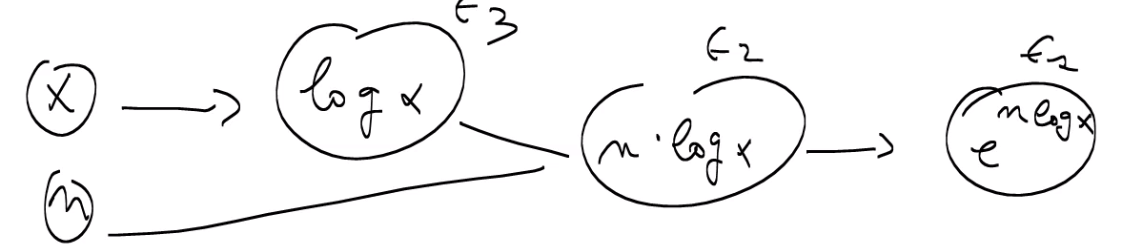
\includegraphics[scale=0.4]{es2_grafo2.png}
\end{center}
$|\epsilon_1| \leq u$, $|\epsilon_2| \leq u$, $|\epsilon_3| \leq u$\\
Per $x \rightarrow \log(x)$ allora $C_x = \frac{\frac{1}{x}}{\log(x)} = \frac{1}{\log(x)}$ ma non amplifica errore su $x$, perché per il calcolo dell'errore algoritmi assumiamo numeri di macchina.\\
Per $x \rightarrow e^x$ allora $C_x = \frac{e^x}{e^x}x = x$. Quindi $\epsilon_2$ ha come coefficiente di amplificazione pari a $n\cdot\log(x)$.\\
Di conseguenza calcolo l'errore algoritmico partendo dalla cima dell'albero e verso le radici (destra verso sinistra) $$\epsilon_{alg} \doteq \epsilon_1 + (n\cdot\log(x))(\epsilon_2 + \epsilon_3)$$
Concludiamo che $|\epsilon_{alg}| = |\epsilon_1 + n\log(x)(\epsilon_2 + \epsilon_3)| \leq |\epsilon_1| + |n\log(x)(\epsilon_2 + \epsilon_3)| \leq u + |n\log(x)|\cdot |\epsilon_2 + \epsilon_3| \leq u + n|\log(x)|(|\epsilon_2| + |\epsilon_3|) \leq u + 2un|\log(x)| = u\cdot(1 + 2\cdot n\cdot|\log(x)|)$ cioè $$|\epsilon_{alg}| \leq u\cdot(1 + 2\cdot n\cdot|\log(x)|)$$ Concludiamo che l'algoritmo è \textbf{numericamente instabile per $x$ piccolo o $x$ è grande}, ma è stabile in un intorno di $1$.\\\\\\\\
L'analisi della stabilità ci dice che il primo algoritmo è preferibile.
\paragraph{Costo computazionale} Il \textbf{primo algoritmo} $\Rightarrow$ $(n - 1)$ operazioni moltiplicative, quindi \textbf{O(n)}.\\
Il \textbf{secondo algoritmo}, più complicato perché ci sono due operazioni non razionali oltre alla moltiplicazione.
\paragraph{Esercizio} Supposto $n = 2^k$ e $f(x) = x^n = x^{2^k}$, determinare un algoritmo che calcola $f(x)$ con $k = \log_2(n)$ operazioni moltiplicative. Eseguire anche l'analisi dell'errore algoritmico per l'algoritmo trovato.
\pagebreak
\section{Matlab}
11 bit esponente rappresentato in traslazione, 52 bit mantissa (53 cifre rappresentabili per il bit nascosto) $\Rightarrow$ $u = B^{1-t} = 2^{-52}$
\subsection{Esponenziale}
$f(x) = e^x$ approssimato con Taylor $$e^x \simeq 1 + x + \frac{x^2}{2} + \frac{x^3}{3!} + \ldots + \frac{x^n}{n!}$$ Implementiamo un algoritmo che dati $x$, $n$ in input restituisce $y = 1 + x + \frac{x^2}{2} + \frac{x^3}{3!} + \ldots + \frac{x^n}{n!}$ in output.\\
Potrebbe essere utile un programma del tipo
\begin{lstlisting}
y = 1;
for k = 1 .. n
	y = y + x^(k)/factorial(k)
end
\end{lstlisting}
Dal punto di vista del costo computazionale, però, ci sono dei problemi. Al passo $k$ faccio $k$ prodotti per $x^k$ e $k$ prodotti per $k!$, quindi \textbf{circa $2k$ prodotti}.\\
Il costo totale è del tipo $C = 2 + 2\cdot 2 + 2\cdot 3 + \ldots + 2\cdot n = 2(1 + 2 + 3 + \ldots + n)$.\\
Ricordiamo $1 + 2 + \ldots + n = \frac{n(n + 1)}{2}$, quindi $C = \not 2\cdot\frac{n(n+1)}{\not 2} =$ O($n^2$) quindi costo quadratico.\\
Una variazione più efficiente
\begin{lstlisting}
y = 1; p = 1; m = 1;
for k = 1 .. n
	p = p * x;	% accumula le potente
	m = m * k;	% accumula il fattoriale
	y = y + p/m	% accumula la somma
end
\end{lstlisting}
Al passo $k$ ho 4 operazioni aritmetiche (o 3 operazioni moltiplicative, perché alcune volte si afferma che $t_* >> t_+$ in termini di operazioni tra bit (\textbf{costo booleano}))\\
Il costo totale $C = 4n$ operazioni (o $3n$).\\
I due algoritmi possono produrre numeri molto grandi. Una versione che argina questo problema è la seguente.
\begin{lstlisting}
y = 1; z = 1;
for k = 1 .. n
	z = z * x/k;	% controllare l'esplosione dei numeri
	y = y + z;
end
\end{lstlisting}
\end{document}
